% !TeX root = ../main.tex
% Add the above to each chapter to make compiling the PDF easier in some editors.

\chapter{Bewertungsdiagramme}\label{chapter:Bewertungsdiagramme}
Abbildung \ref{fig:Bewertung_UTF(2)} stellt einen Ausschnitt der Abbildung \ref{fig:Bewertung_UTF} mit dem Häufigkeitsbereich 0 bis 11 \% dar. Die Häufigkeiten der Unfalltypen, bei denen es zu einem Kleinunfall, schwerwiegendem Sachschaden im engeren Sinne oder einer leichten Verletzung kam, sind so deutlicher zu erkennen. Ein weiterer Ausschnitt in derselben Abbildung verdeutlicht die Häufigkeiten der Unfalltypen, bei denen Personen schwer verletzt wurden.

\begin{savenotes}
	\begin{figure}[H]
		\centering
		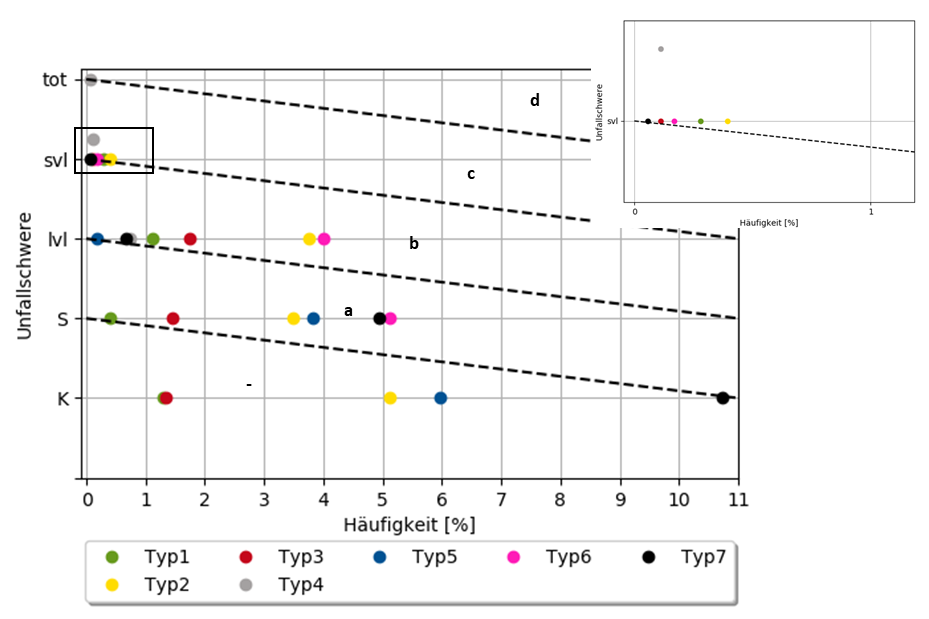
\includegraphics[width=12cm,height=8cm]{figures/Bewertung_UTF(2)}
		\caption[Bewertung der Unfälle im Testgebiet anhand der sieben Unfalltypen ohne Typ 6 bei den Kleinunfällen]{Bewertung der Unfälle im Testgebiet anhand der sieben Unfalltypen ohne Typ 6 bei den Kleinunfällen}\label{fig:Bewertung_UTF(2)}
	\end{figure}
\end{savenotes}

In Abbildung \ref{fig:Bewertung_FT6(2)} wird ein Ausschnitt der Abbildung \ref{fig:Bewertung_FT6} dargestellt.

\begin{savenotes}
	\begin{figure}[H]
		\centering
		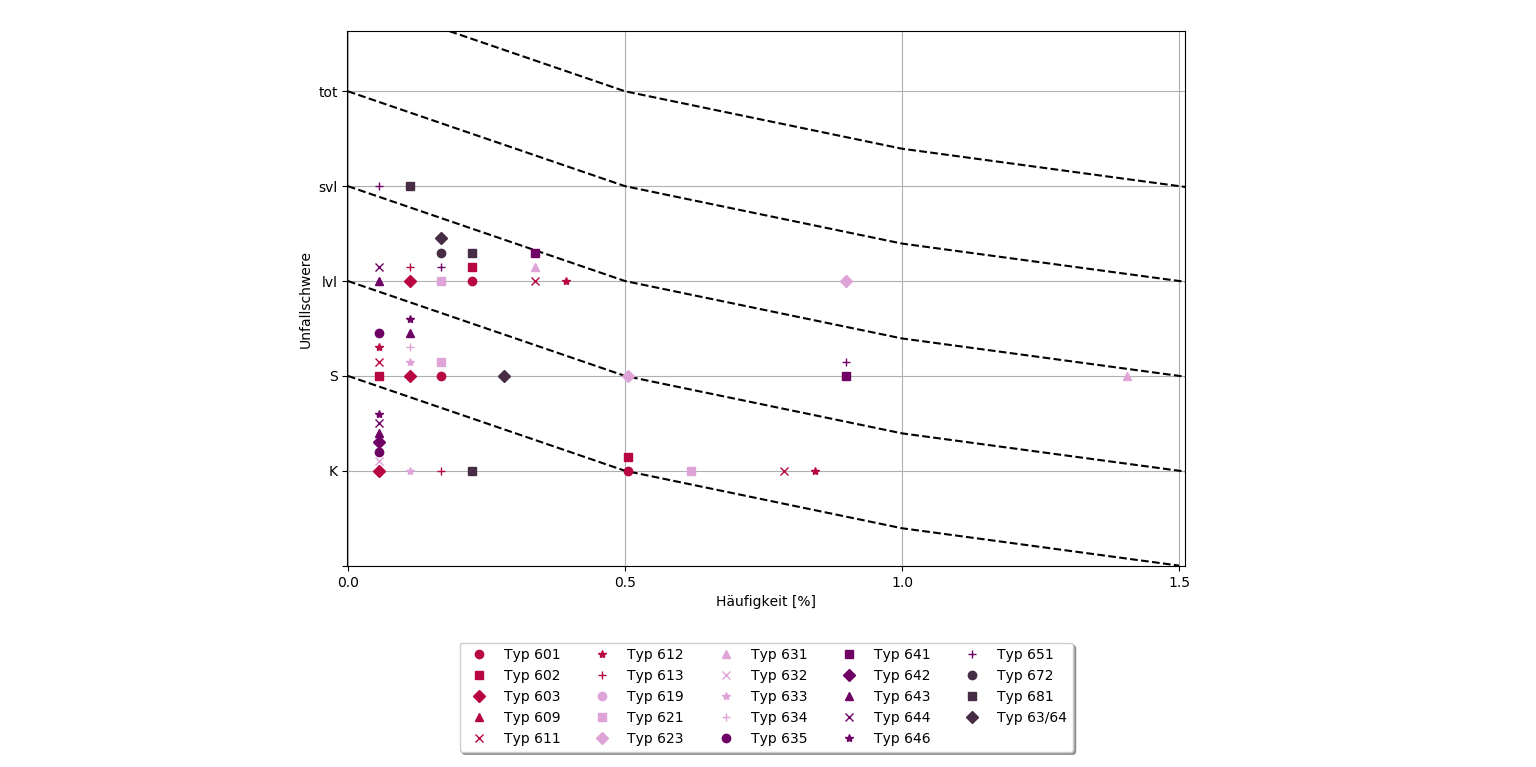
\includegraphics[width=13.5cm,height=9cm]{figures/Bewertung_FT6(2)}
		\caption[Ausschnitt aus der Bewertung der Unfälle, denen ein Feintyp des Unfalltyps 6 zugeordnet wurde]{Ausschnitt aus der Bewertung der Unfälle, denen ein Feintyp des Unfalltyps 6 zugeordnet wurde}\label{fig:Bewertung_FT6(2)}
	\end{figure}
\end{savenotes}